\chapter{Evaluation}
\label{chapter:evaluation}

\guidance{%
  This is where Assessors will be looking for \textbf{signs of success} and for
  \textbf{evidence of thorough and systematic testing}. \textbf{Sample output},
  tables of timings and photographs of workstation screens, oscilloscope traces
  or circuit boards may be included.\\
  As with code, voluminous examples of sample output are usually best left to
  appendices or omitted altogether.\\
  There are some obvious questions which this chapter will address. \textbf{How
  many of the original goals were achieved? Were they proved to have been
  achieved? Did the program, hardware, or theory really work?}\\
  Assessors are well aware that large programs will very likely include some
  residual bugs. It should always be possible to demonstrate that a
  \textbf{program works in simple cases} and it is instructive to
  \textbf{demonstrate how close it is to working in a really ambitious case}.\\
}

\prechapter{%
  Here, the project's resounding success, in relation to the aims of the project
  (as listed in Section~\ref{intro:aims}), will be justified. A comparison with
  existing tools will demonstrate the advantages of this project over existing
  tools (those mentioned in Subsection~\ref{prep:coqtools}). Sample output will
  be shown and the interesting insights they provide will be explained. 
}%

\begin{figure}[tbp]

  \raggedright
  This project aims to:

  \begin{itemize}
  \item represent Coq libraries as Neo4j graph databases, which wil involve
    \begin{itemize}
    \item exploring and choosing the correct model
    \item converting and extending existing code to output CSVs
    \item writing new programs to extract extra information \\
        (omitted from other, existing tools)
    \item writing new programs to automate database creation; and to
    \end{itemize}

  \item create a library of Neo4j queries, intended
    \begin{itemize}
    \item to highlight the structure of and relationship between proof-objects
    \item by coalescing and implementing several graph-related metrics.
    \end{itemize}
  \end{itemize}

  \hrule%
  \caption{Aims of the Project}\label{fig:aims}

\end{figure}

\section{Capabilities}\label{eval:compare}

For convenience, the aims of the project, as listed in
Section~\ref{intro:aims}, are reproduced above, in Figure~\ref{fig:aims}.
Within the first major bullet-point (representing Coq libraries as Neo4j
databases), the latter three aims (of adapting, extending and writing new
programs to output CSV, extracting extra information and automating database
creation) were exposited in the~\nameref{chap:impl} chapter.

So, to assess the first aim of the project (exploring and choosing the
correct model), all of the programs listed in
Subsection~\ref{prep:coqtools},~\nameref{prep:coqtools}, are compared
side-by-side in Table~\ref{table:features}, in which this project comes out
favourably. Performance (specifically, the time to set up a database from
scratch) is also considered, to demonstrate that the project is usable on large
mathematical theories. 

\subsection{Features Supported by Other Tools}

\begin{table}[p]
\centering

\begin{tabular*}{\textwidth}{@{\extracolsep{\fill}} rcccccccccc}

  \toprule

  &
  \rot{Source Code} &
  \rot{Hyperlinks} &
  \rot{Precise Kinds} &
  \rot{Constr. \& Types~~} & % for vertical space after 'Types'
  \rot{Type Sig.} &
  \rot{Module depend.} &
  \rot{Graphical rep.} &
  \rot{Interactivity} &
  \rot{Statistics} &
  \rot{Object depend.} \\

  \midrule

  Coqdoc    & \Y & \Y & \Y & \Y & \Y & \N & \N & \N & \N & \N \\
  Coqdep    & \N & \M & \N & \N & \N & \Y & \Y & \N & \N & \N \\
  CoqSerAPI & \N & \N & \N & \N & \N & \N & \N & \Y & \Y & \N \\
  dpdgraph  & \N & \N & \M & \N & \N & \N & \Y & \N & \N & \Y \\
  Project   & \M & \Y & \Y & \Y & \Y & \Y & \Y & \Y & \Y & \Y \\

  \bottomrule

\end{tabular*}

\medskip
\Y\  Has feature \hfill \N\ Does not have feature \hfill \M\ Can be extended to support it

\bigskip
\caption{Comparison of Features}\label{table:features}

\end{table}

The features chosen for comparison reflect the strengths of each tool
considered.

Bundle with Coq, coqdoc produces \textbf{hyperlinked source code} meaning
details such as the \textbf{precise kinds} of a proof-object, the
\textbf{constructors of a type} and the \textbf{type signatures} are immediately
visible; hence those 5 dimensions were included.  Also include in a Coq system
is coqdep: a tool for modelling \textbf{module-level dependencies} that can
output a \texttt{dot} file to present it \textbf{graphically}.

Coq Serialised (S-expression) API is an \textbf{interactive} IDE communication
protocol with facilities for gathering some basic \textbf{statistics}. Here,
interative is used to mean that information is not presented all at-once,
\emph{statically}, but can instead by queried dynamically at run-time. An
example of a static dispaly is Figure~\ref{fig:static}; it shows is a SVG
(scalable vector-graphic) output by dpdgraph of a medium-size Coq library.

\begin{figure}[p]

  \centering
  \includegraphics[width=\textwidth, page=1]{img/static-CAS-small.pdf}
  \caption{Static Output of dpdgraph (using \texttt{dpd2dot}) on
    \href{https://github.com/Timothy-G-Griffin/CAS}{CAS}}\label{fig:static}

\end{figure}

In principle, coqdep and dpdgraph can also support some degree of interactivity,
with support from other tools (which translate \texttt{dot} files to interactive
JavaScript), although this is rarely done.  What dpdgraph does do well is model
\textbf{object dependencies}, with some scope for distinguishing precise kinds
and displaying information graphically.

\subsection{Features Supported by this Project}

It is clear from the table that this project either supports, or can support,
every feature supported by other tools. However, it is important to note, that
in many cases, this project does not simply match the feature, but exceeds it in
ways described next.

Linking to source code could be supported by modifying either the model,
database or JavaScript visualisations (outuput by the library of queries) to
link to the relevant webpages output by coqdoc. So, a user could switch between
a graphical overview and a detailed inspection at will.

Whenever a node is visible, it can be expanded to see the nodes it depends on,
so in that sense, it supports hyperlinks, though, unlike hyperlinks, such
expansion is done in place, thus retaining the \emph{context} of its use.

Thanks to the \emph{kind} and \emph{subkind} labels, the project supports
precise kinds.  Also, any (co-)inductive type can, via the
\texttt{CONSTRUCTED\_BY} relation, be expanded to see its constructors. 

Due to the \emph{type} property, each object's type is also visible. For a proof
object, its type is a statement of the actual theorem being proved, hence this
feature is incredibly important when coming to grips with a mathematical theory.
Crucially, it is a \emph{fully expanded} type signature, making explicit any
assumptions introduced (perhaps hunderds of lines prior in the source code) into
the environment.

Module dependencies are set with the query in Listing~\ref{lst:moddep} by use of
the \texttt{CONTAINS} relation.  Interactivity is achieved through the Neo4j
browser interface and the JavaScript visualisations; statistics are achieved
through the library of queries; graphical representations by both. An important
limitation of CoqSerAPI is that its statistics are (at the time of writing)
simply three counters, whereas this project offers many sophisticated graph
metrics and the ability (through a queriable database) to gain \emph{any} sort
of information a user is interested in.

\begin{listing}[p]%

\caption{Query to set Module Dependencies}\label{lst:moddep}

  \begin{minted}{cypher}
    MATCH (a)-[:USES]->(b),
          (src:module)-[:CONTAINS]->(a),
          (dst:module)-[:CONTAINS]->(b)
    WHERE src.objectId <> dst.objectId
    CREATE UNIQUE (src)-[r:DEPENDS_ON]->(dst)
    SET r.weight = coalesce(r.weight, 0) + 1
    RETURN r
  \end{minted}

\end{listing}

And finally, object dependencies are at the heart of this project: by using a
Neo4j graph database, we can understand and manipulate this relation in a much
more flexible and scalable manner than any visualisation can manage.

\subsection{Performance}

Setting up a graph database from scratch can take some time. Assuming a Coq project
is already compiled, the following steps need to take place:

\begin{enumerate}
  \item write file with a list of all the modules to be examined,
  \item compile that file using the Coq compiler,
  \item convert the output \texttt{dpd} file to CSV files,
  \item create a Neo4j database from those CSV files
  \item and run the R library scripts over the newly-instantiated databases.
\end{enumerate}

And finally, object dependencies are at the heart of this project: by using a
Neo4j graph database, we can understand and manipulate this relation in a much
more flexible and scalable manner than any visualisation can manage.

\begin{figure}[p]
\centering

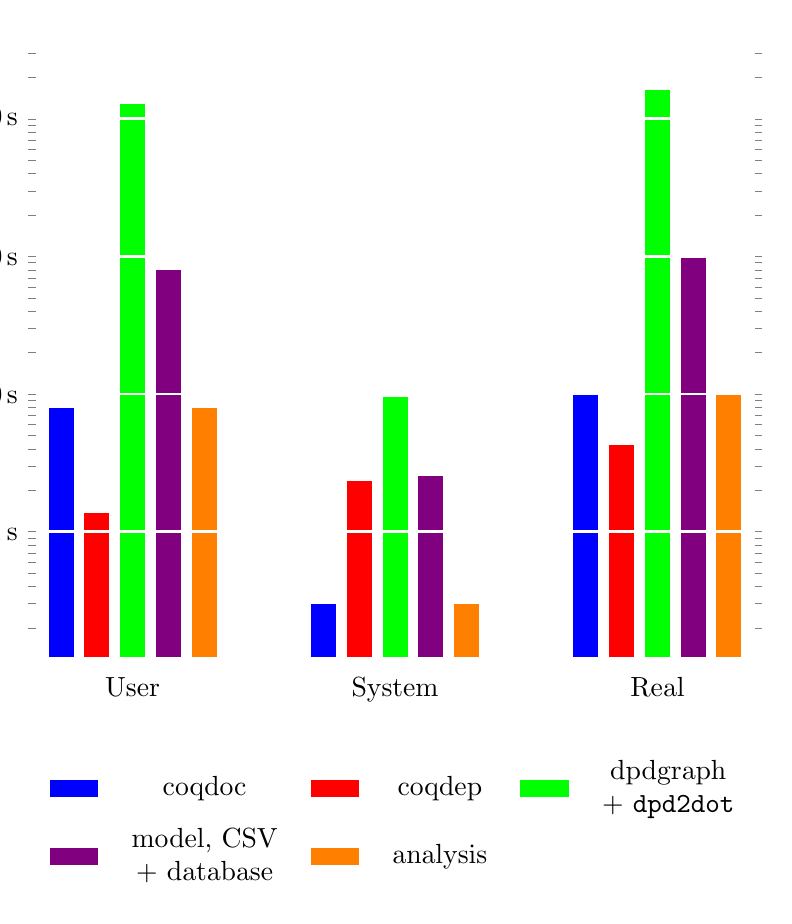
\begin{tikzpicture}[trim axis left]
	\begin{axis}[
    % width of chart
    width=0.9\textwidth,
    % no box, below chart, horizontal
		legend style={%
      draw=none,
      at={(0.5,-0.15)},
      anchor=north,
      legend columns=3,
      column sep = 1em,
      cells={align=center},
    },
    % value above position on bar chart
		ybar=1ex, % bar chart, with inter-bar spacing of 1ex
    log ticks with fixed point,
    yticklabel={\pgfmathparse{pow(10,\tick-3)}\pgfmathprintnumber[fixed]{\pgfmathresult}}\,s, % N ms along y-axis
    symbolic x coords={User,System,Real},
		xtick=data,
    axis line style={opacity=0}, % hide y axis
    major tick style={draw=none}, % no ticks
    ymin = 0,
    ymode=log, % log scale for y
    log basis y = {10}, % log base 10
		enlarge x limits=0.20, % spacing on x axis
    bar width=2ex,
    ymajorgrids, % rows of lines
    major grid style={white, line width=1pt},
    axis on top,
	]

  % Coqdoc
  \addplot [area legend, style={blue,fill=blue,mark=none}]
    coordinates {(User,7877) (System,0295) (Real,10007)};

  % Coqdep
  \addplot [area legend, style={red,fill=red,mark=none}]
    coordinates {(User,1361) (System,2299) (Real,4257)};

  % dpdgraph + dpd2dot
  \addplot [area legend, style={green,fill=green,mark=none}]
    coordinates {(User,1279121) (System,9388) (Real,1597695)};

  % creation
  \addplot [area legend, style={violet,fill=violet,mark=none}]
    coordinates {(User,79254) (System,2521) (Real,98157)};

  % analysis
  \addplot [area legend, style={orange,fill=orange,mark=none}]
    coordinates {(User,7877) (System,0295) (Real,10007)};

  \legend{coqdoc,coqdep,dpdgraph\\+ \texttt{dpd2dot},{model, CSV\\+ database},analysis}

	\end{axis}

\end{tikzpicture}

\caption{Comparison of Execution Times}\label{fig:exectimes}

\end{figure}

\section{Library of Queries}\label{sec:libeval}

Due to the \emph{type} property, each object's type is also visible. For a proof
object, its type is a statement of the actual theorem being proved, hence this
feature is incredibly important when coming to grips with a mathematical theory.
Crucially, it is a \emph{fully expanded} type signature, making explicit any
assumptions introduced (perhaps hunderds of lines prior in the source code) into
the environment.

Module dependencies are set with the query in Listing~\ref{lst:moddep} by use of
the \texttt{CONTAINS} relation.  Interactivity is achieved through the Neo4j
browser interface and the JavaScript visualisations; statistics are achieved
through the library of queries; graphical representations by both. An important
limitation of CoqSerAPI is that its statistics are simply three counters,
whereas this project offers the ability, through a queriable database, to gain
\emph{any} sort of information a user is interested in.

And finally, object dependencies are at the heart of this project: by using a
Neo4j graph database, we can understand and manipulate this relation in a much
more flexible and scalable manner than any visualisation can manage.

\subsection{Small: CoqRegExp}

Due to the \emph{type} property, each object's type is also visible. For a proof
object, its type is a statement of the actual theorem being proved, hence this
feature is incredibly important when coming to grips with a mathematical theory.
Crucially, it is a \emph{fully expanded} type signature, making explicit any
assumptions introduced (perhaps hunderds of lines prior in the source code) into
the environment.

Module dependencies are set with the query in Listing~\ref{lst:moddep} by use of
the \texttt{CONTAINS} relation.  Interactivity is achieved through the Neo4j
browser interface and the JavaScript visualisations; statistics are achieved
through the library of queries; graphical representations by both. An important
limitation of CoqSerAPI is that its statistics are simply three counters,
whereas this project offers the ability, through a queriable database, to gain
\emph{any} sort of information a user is interested in.

And finally, object dependencies are at the heart of this project: by using a
Neo4j graph database, we can understand and manipulate this relation in a much
more flexible and scalable manner than any visualisation can manage.

\subsection{Large: MathComp}

Due to the \emph{type} property, each object's type is also visible. For a proof
object, its type is a statement of the actual theorem being proved, hence this
feature is incredibly important when coming to grips with a mathematical theory.
Crucially, it is a \emph{fully expanded} type signature, making explicit any
assumptions introduced (perhaps hunderds of lines prior in the source code) into
the environment.

Module dependencies are set with the query in Listing~\ref{lst:moddep} by use of
the \texttt{CONTAINS} relation.  Interactivity is achieved through the Neo4j
browser interface and the JavaScript visualisations; statistics are achieved
through the library of queries; graphical representations by both. An important
limitation of CoqSerAPI is that its statistics are simply three counters,
whereas this project offers the ability, through a queriable database, to gain
\emph{any} sort of information a user is interested in.

And finally, object dependencies are at the heart of this project: by using a
Neo4j graph database, we can understand and manipulate this relation in a much
more flexible and scalable manner than any visualisation can manage.

